\documentclass[aspectratio=169,10pt]{beamer}

\usepackage[T1]{fontenc}
\usepackage{lmodern}
\usepackage{amsmath,amssymb,booktabs,array}
\usepackage{graphicx}
\usepackage{tikz}
\usetikzlibrary{arrows.meta,calc,positioning,fit,backgrounds,shapes.geometric}
\pgfmathsetseed{7}

\definecolor{ink}{HTML}{17212B}
\definecolor{muted}{HTML}{68737D}
\definecolor{teal}{HTML}{008B8B}
\definecolor{blue}{HTML}{376C9F}
\definecolor{orange}{HTML}{E36F35}
\definecolor{gold}{HTML}{D4A72C}
\definecolor{red}{HTML}{C14953}
\definecolor{green}{HTML}{3B8C6E}
\definecolor{violet}{HTML}{7656A6}
\definecolor{paper}{HTML}{F7F8F8}
\definecolor{line}{HTML}{D9DEE2}

\setbeamercolor{normal text}{fg=ink,bg=white}
\setbeamercolor{frametitle}{fg=ink,bg=white}
\setbeamercolor{structure}{fg=teal}
\setbeamercolor{alerted text}{fg=orange}
\setbeamertemplate{navigation symbols}{}
\setbeamertemplate{headline}{}
\setbeamertemplate{footline}{%
  \leavevmode\hbox to \paperwidth{\hspace*{0.45cm}\color{muted}\scriptsize Rafael F. Schaefer \enspace|\enspace Generative Channel Modeling\hfill\insertframenumber\hspace*{0.45cm}}\vspace{0.16cm}}
\setbeamertemplate{frametitle}{\vspace{0.28cm}\hspace{-0.1cm}\insertframetitle\par\vspace{0.12cm}\color{line}\rule{\textwidth}{0.45pt}}
\setbeamertemplate{itemize item}{\color{teal}\raise0.15ex\hbox{\small$\blacktriangleright$}}
\setbeamertemplate{itemize subitem}{\color{muted}\raise0.1ex\hbox{\scriptsize$\bullet$}}
\setbeamerfont{frametitle}{size=\Large,series=\bfseries}
\setbeamerfont{title}{size=\LARGE,series=\bfseries}
\setbeamerfont{subtitle}{size=\large}

\newcommand{\pill}[2]{\tikz[baseline=-0.6ex]\node[fill=#1!10,draw=#1!45,rounded corners=2pt,inner xsep=7pt,inner ysep=3pt,text=#1,font=\scriptsize\bfseries]{#2};}
\newcommand{\softbox}[2]{\begin{tikzpicture}\node[fill=#1!7,draw=#1!35,rounded corners=3pt,inner sep=8pt,text width=0.9\linewidth]{#2};\end{tikzpicture}}
\newcommand{\method}[2]{\tikz[baseline=-0.65ex]\node[circle,fill=#1,minimum size=1.25ex,inner sep=0pt]{};\,#2}
\newcommand{\sourcefig}[1]{assets/#1}
\newcommand{\slideref}[1]{\par\vspace{0.12cm}{\raggedright\tiny\color{muted}#1\par}}

\title{From GANs to Diffusion and Drifting}
\subtitle{Generative Channel Models for 6G}
\author{Rafael F. Schaefer \and Rick Fritschek}
\institute{Chair of Information Theory and Machine Learning\\TUD Dresden University of Technology}
\date{}

\begin{document}

% 1
\begin{frame}[plain]
\vspace{0.35cm}
{\usebeamerfont{title}\color{ink}\inserttitle\par}
\vspace{0.10cm}
{\usebeamerfont{subtitle}\color{teal}\insertsubtitle\par}
\vspace{0.28cm}
{\small Rafael F. Schaefer \quad Rick Fritschek\par}
\vspace{0.06cm}
{\scriptsize\color{muted} Chair of Information Theory and Machine Learning, TUD Dresden University of Technology\par}
\vspace{0.78cm}
\centering
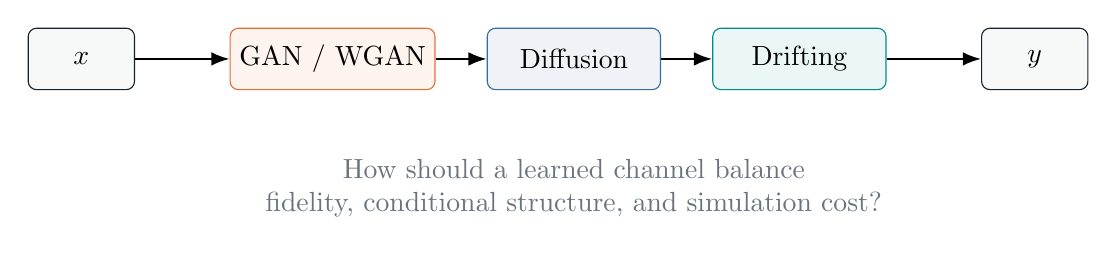
\begin{tikzpicture}[>=Latex, node distance=1.15cm]
  \node[draw=ink,fill=paper,rounded corners=3pt,minimum width=1.35cm,minimum height=0.78cm] (x) {$x$};
  \node[draw=orange,fill=orange!8,rounded corners=3pt,minimum width=2.2cm,minimum height=0.78cm,right=1.2cm of x] (w) {GAN / WGAN};
  \node[draw=blue,fill=blue!8,rounded corners=3pt,minimum width=2.2cm,minimum height=0.78cm,right=0.65cm of w] (d) {Diffusion};
  \node[draw=teal,fill=teal!8,rounded corners=3pt,minimum width=2.2cm,minimum height=0.78cm,right=0.65cm of d] (r) {Drifting};
  \node[draw=ink,fill=paper,rounded corners=3pt,minimum width=1.35cm,minimum height=0.78cm,right=1.2cm of r] (y) {$y$};
  \draw[->,thick] (x)--(w); \draw[->,thick] (w)--(d); \draw[->,thick] (d)--(r); \draw[->,thick] (r)--(y);
  \node[below=0.75cm of d,align=center,text=muted] {How should a learned channel balance\\fidelity, conditional structure, and simulation cost?};
\end{tikzpicture}
\vfill
\pill{blue}{FIDELITY}\quad\pill{orange}{CONDITIONING}\quad\pill{green}{DIFFERENTIABLE}\quad\pill{teal}{FAST SAMPLING}
\end{frame}

% 2
\begin{frame}{A learned channel is a conditional sampler}
\begin{columns}[T,onlytextwidth]
\column{0.48\textwidth}
\centering
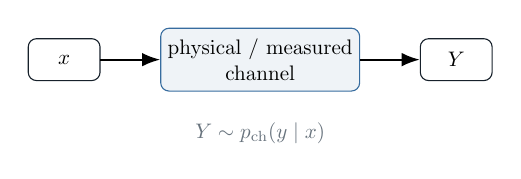
\begin{tikzpicture}[>=Latex,node distance=0.8cm,scale=0.76,transform shape]
\node[draw=ink,rounded corners=3pt,minimum width=1.2cm,minimum height=0.7cm] (x) {$x$};
\node[draw=blue,fill=blue!8,rounded corners=3pt,minimum width=3.1cm,minimum height=1.05cm,right=1cm of x,align=center] (ch) {physical / measured\\channel};
\node[draw=ink,rounded corners=3pt,minimum width=1.2cm,minimum height=0.7cm,right=1cm of ch] (y) {$Y$};
\draw[->,thick] (x)--(ch); \draw[->,thick] (ch)--(y);
\node[below=0.4cm of ch,text=muted] {$Y\sim p_{\mathrm{ch}}(y\mid x)$};
\end{tikzpicture}
\vspace{0.6cm}
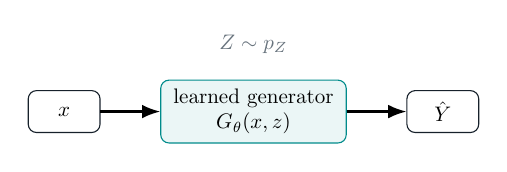
\begin{tikzpicture}[>=Latex,node distance=0.8cm,scale=0.76,transform shape]
\node[draw=ink,rounded corners=3pt,minimum width=1.2cm,minimum height=0.7cm] (x) {$x$};
\node[draw=teal,fill=teal!8,rounded corners=3pt,minimum width=3.1cm,minimum height=1.05cm,right=1cm of x,align=center] (g) {learned generator\\$G_\theta(x,z)$};
\node[draw=ink,rounded corners=3pt,minimum width=1.2cm,minimum height=0.7cm,right=1cm of g] (y) {$\hat Y$};
\node[above=0.32cm of g,text=muted] {$Z\sim p_Z$};
\draw[->,thick] (x)--(g); \draw[->,thick] (g)--(y);
\end{tikzpicture}
\column{0.48\textwidth}
\vspace{0.25cm}
\begin{block}{The target}
\centering\large
$p_{G_\theta(X,Z)\mid X}(\cdot\mid x)\ \approx\ p_{\mathrm{ch}}(\cdot\mid x)$
\end{block}
\vspace{0.35cm}
\begin{itemize}\setlength\itemsep{0.45em}
\item nonlinear and mismatched hardware
\item data-driven channel characterization
\item differentiable end-to-end learning
\item repeated Monte Carlo simulation
\end{itemize}
\end{columns}
\end{frame}

% 3
\begin{frame}{A useful simulator must satisfy four constraints}
\centering
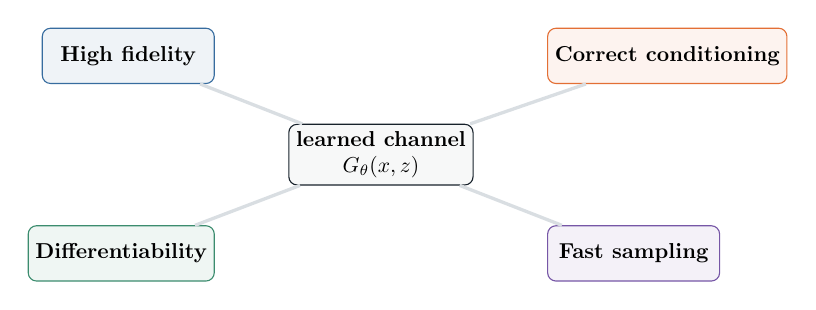
\begin{tikzpicture}[node distance=0.75cm,scale=0.78,transform shape]
\node[draw=ink,fill=paper,rounded corners=3pt,minimum width=2.8cm,minimum height=0.95cm,align=center,font=\bfseries] (c) {learned channel\\$G_\theta(x,z)$};
\node[draw=blue,fill=blue!8,rounded corners=3pt,minimum width=2.8cm,minimum height=0.9cm,above left=0.65cm and 1.2cm of c,align=center,font=\bfseries] (a) {High fidelity};
\node[draw=orange,fill=orange!8,rounded corners=3pt,minimum width=2.8cm,minimum height=0.9cm,above right=0.65cm and 1.2cm of c,align=center,font=\bfseries] (b) {Correct conditioning};
\node[draw=green,fill=green!8,rounded corners=3pt,minimum width=2.8cm,minimum height=0.9cm,below left=0.65cm and 1.2cm of c,align=center,font=\bfseries] (d) {Differentiability};
\node[draw=violet,fill=violet!8,rounded corners=3pt,minimum width=2.8cm,minimum height=0.9cm,below right=0.65cm and 1.2cm of c,align=center,font=\bfseries] (e) {Fast sampling};
\foreach \n in {a,b,d,e} \draw[-,line width=1.2pt,line] (c)--(\n);
\end{tikzpicture}
\vspace{0.45cm}
\begin{columns}[T,onlytextwidth]
\column{0.24\textwidth}
\centering
\begin{tikzpicture}\node[fill=blue!9,draw=blue!45,rounded corners=3pt,text width=0.85\linewidth,minimum height=1.25cm,align=center,inner sep=6pt,font=\scriptsize] {Match distribution shape, variability, and relevant tails.};\end{tikzpicture}
\column{0.24\textwidth}
\centering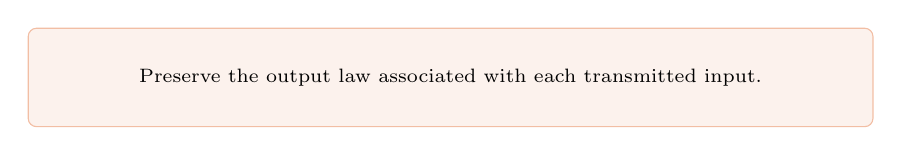
\begin{tikzpicture}\node[fill=orange!9,draw=orange!45,rounded corners=3pt,text width=0.85\linewidth,minimum height=1.25cm,align=center,inner sep=6pt,font=\scriptsize] {Preserve the output law associated with each transmitted input.};\end{tikzpicture}
\column{0.24\textwidth}
\centering
\begin{tikzpicture}\node[fill=green!9,draw=green!45,rounded corners=3pt,text width=0.85\linewidth,minimum height=1.25cm,align=center,inner sep=6pt,font=\scriptsize] {Allow optimization through the learned channel response.};\end{tikzpicture}
\column{0.24\textwidth}
\centering
\begin{tikzpicture}\node[fill=violet!9,draw=violet!45,rounded corners=3pt,text width=0.85\linewidth,minimum height=1.25cm,align=center,inner sep=6pt,font=\scriptsize] {Keep repeated training and Monte Carlo calls affordable.};\end{tikzpicture}
\end{columns}
\end{frame}

% 4
\begin{frame}{GANs offer direct samples; WGAN is our baseline}
\textcolor{teal}{\bfseries INFERENCE}\par\vspace{0.18cm}
\begin{columns}[c,onlytextwidth]
\column{0.58\textwidth}
\centering
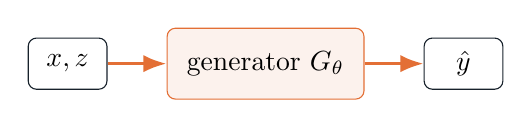
\begin{tikzpicture}[>=Latex,node distance=0.75cm]
\node[draw=ink,rounded corners=3pt,minimum width=1cm,minimum height=0.65cm] (z) {$x,z$};
\node[draw=orange,fill=orange!9,rounded corners=3pt,minimum width=2.5cm,minimum height=0.9cm,right=of z] (g) {generator $G_\theta$};
\node[draw=ink,rounded corners=3pt,minimum width=1cm,minimum height=0.65cm,right=of g] (y) {$\hat y$};
\draw[->,very thick,orange] (z)--(g); \draw[->,very thick,orange] (g)--(y);
\end{tikzpicture}
\column{0.38\textwidth}
\large Direct conditional generation\par
\smallskip
\textcolor{teal}{\bfseries one generator evaluation}
\end{columns}

\vspace{0.35cm}
{\color{line}\rule{\textwidth}{0.45pt}}
\vspace{0.25cm}

\textcolor{orange}{\bfseries TRAINING}\par\vspace{0.16cm}
\begin{columns}[c,onlytextwidth]
\column{0.52\textwidth}
\centering
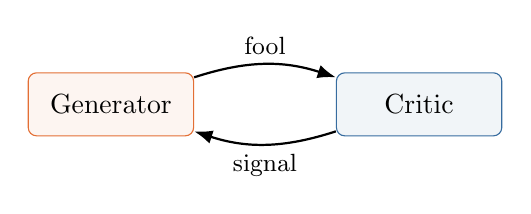
\begin{tikzpicture}[>=Latex,node distance=1cm]
\node[draw=orange,fill=orange!7,rounded corners=3pt,minimum width=2.1cm,minimum height=0.8cm] (g) {Generator};
\node[draw=blue,fill=blue!7,rounded corners=3pt,minimum width=2.1cm,minimum height=0.8cm,right=1.8cm of g] (c) {Critic};
\draw[->,thick,bend left=18] (g) to node[above,font=\small]{fool} (c);
\draw[->,thick,bend left=18] (c) to node[below,font=\small]{signal} (g);
\end{tikzpicture}
\column{0.44\textwidth}
\begin{itemize}\setlength\itemsep{0.28em}
\item adversarial min--max optimization
\item stability and balance
\item distribution coverage
\end{itemize}
\end{columns}
\slideref{I. Goodfellow et al., NeurIPS 2014. M. Arjovsky et al., ICML 2017. The experiments in this talk use a conditional WGAN baseline.}
\end{frame}

% 5
\begin{frame}{GAN channel models established the differentiable-surrogate idea}
\begin{columns}[T,onlytextwidth]
\column{0.32\textwidth}
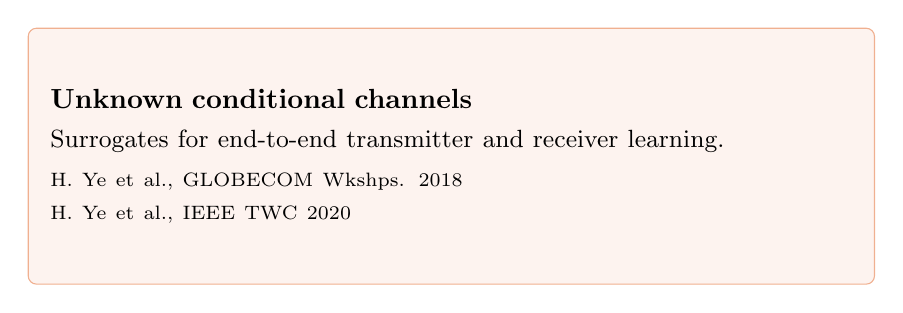
\begin{tikzpicture}
\node[draw=orange!55,fill=orange!8,rounded corners=3pt,text width=0.84\linewidth,minimum height=3.25cm,align=left,inner sep=8pt] {
\textbf{Unknown conditional channels}\par\smallskip
\small Surrogates for end-to-end transmitter and receiver learning.\par\medskip
\scriptsize H. Ye et al., GLOBECOM Wkshps. 2018\par
H. Ye et al., IEEE TWC 2020};
\end{tikzpicture}
\column{0.32\textwidth}
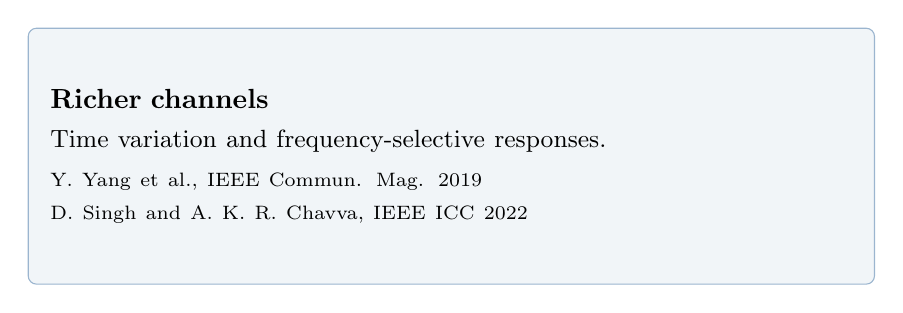
\begin{tikzpicture}
\node[draw=blue!50,fill=blue!7,rounded corners=3pt,text width=0.84\linewidth,minimum height=3.25cm,align=left,inner sep=8pt] {
\textbf{Richer channels}\par\smallskip
\small Time variation and frequency-selective responses.\par\medskip
\scriptsize Y. Yang et al., IEEE Commun. Mag. 2019\par
D. Singh and A. K. R. Chavva, IEEE ICC 2022};
\end{tikzpicture}
\column{0.32\textwidth}
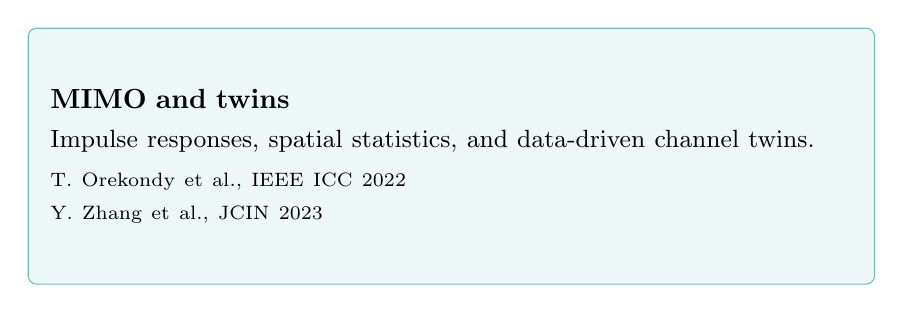
\begin{tikzpicture}
\node[draw=teal!55,fill=teal!7,rounded corners=3pt,text width=0.84\linewidth,minimum height=3.25cm,align=left,inner sep=8pt] {
\textbf{MIMO and twins}\par\smallskip
\small Impulse responses, spatial statistics, and data-driven channel twins.\par\medskip
\scriptsize T. Orekondy et al., IEEE ICC 2022\par
Y. Zhang et al., JCIN 2023};
\end{tikzpicture}
\end{columns}
\vspace{0.55cm}
\centering

\begin{tikzpicture}[>=Latex]
\node[text=orange,font=\bfseries] (a) {conditional surrogate};
\node[text=blue,font=\bfseries,right=1.25cm of a] (b) {channel memory};
\node[text=teal,font=\bfseries,right=1.25cm of b] (c) {spatial structure};
\draw[->,thick,muted] (a)--(b); \draw[->,thick,muted] (b)--(c);
\end{tikzpicture}
\end{frame}

% 6
\begin{frame}{Diffusion learns difficult channel laws through denoising}
\centering
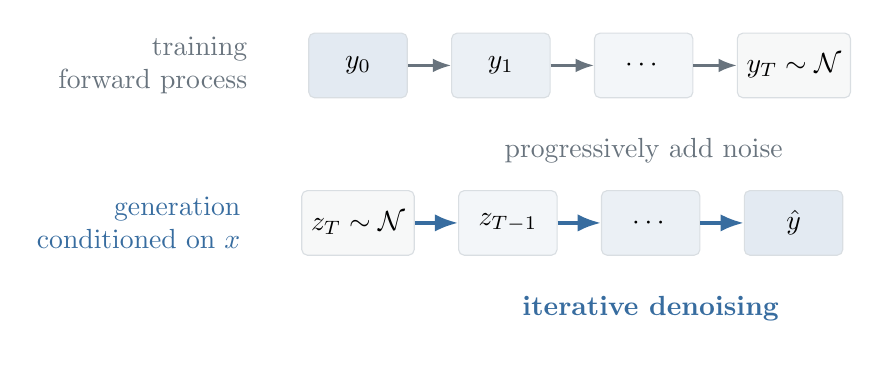
\begin{tikzpicture}[>=Latex, every node/.style={minimum width=1.25cm,minimum height=0.82cm,rounded corners=2pt,draw=line}]
\node[fill=blue!14] (y0) {$y_0$};
\node[fill=blue!10,right=0.55cm of y0] (y1) {$y_1$};
\node[fill=blue!6,right=0.55cm of y1] (y2) {$\cdots$};
\node[fill=paper,right=0.55cm of y2] (yt) {$y_T\sim\mathcal N$};
\draw[->,thick,muted] (y0)--(y1); \draw[->,thick,muted] (y1)--(y2); \draw[->,thick,muted] (y2)--(yt);
\node[left=0.65cm of y0,draw=none,text=muted,align=right] {training\\forward process};
\node[draw=none,below=0.25cm of y2,text=muted] {progressively add noise};
\begin{scope}[yshift=-2.0cm]
\node[fill=paper] (z) {$z_T\sim\mathcal N$};
\node[fill=blue!6,right=0.55cm of z] (z2) {$z_{T-1}$};
\node[fill=blue!10,right=0.55cm of z2] (z1) {$\cdots$};
\node[fill=blue!14,right=0.55cm of z1] (yy) {$\hat y$};
\draw[->,very thick,blue] (z)--(z2); \draw[->,very thick,blue] (z2)--(z1); \draw[->,very thick,blue] (z1)--(yy);
\node[left=0.65cm of z,draw=none,text=blue,align=right] {generation\\conditioned on $x$};
\node[draw=none,below=0.25cm of z1,text=blue,font=\bfseries] {iterative denoising};
\end{scope}
\end{tikzpicture}
\vfill
\begin{columns}[onlytextwidth]
\column{0.48\textwidth}\centering\pill{blue}{STRENGTH}\quad strong distributional modeling
\column{0.48\textwidth}\centering\pill{orange}{COST}\quad sequential generation
\end{columns}
\slideref{J. Ho et al., NeurIPS 2020. J. Song et al., ICLR 2021. M. Kim et al., IEEE ICC 2024.}
\end{frame}

% 7
\begin{frame}{Diffusion reset the fidelity benchmark for image generation}
\begin{columns}[T,onlytextwidth]
\column{0.54\textwidth}
\vspace{0.15cm}
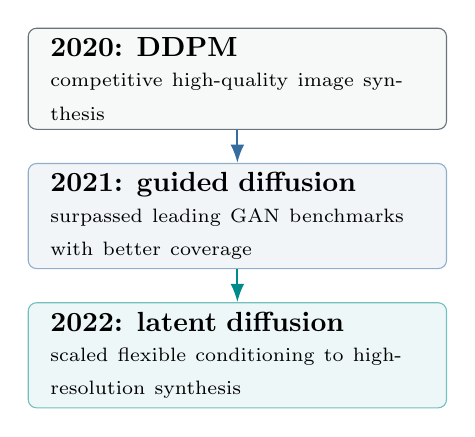
\begin{tikzpicture}[>=Latex,node distance=0.42cm]
\node[draw=muted,fill=paper,rounded corners=3pt,minimum width=5.25cm,minimum height=0.82cm,align=left,text width=4.75cm,inner xsep=8pt] (a) {\textbf{2020: DDPM}\\[-1pt]\scriptsize competitive high-quality image synthesis};
\node[draw=blue!55,fill=blue!7,rounded corners=3pt,minimum width=5.25cm,minimum height=0.82cm,below=of a,align=left,text width=4.75cm,inner xsep=8pt] (b) {\textbf{2021: guided diffusion}\\[-1pt]\scriptsize surpassed leading GAN benchmarks with better coverage};
\node[draw=teal!55,fill=teal!7,rounded corners=3pt,minimum width=5.25cm,minimum height=0.82cm,below=of b,align=left,text width=4.75cm,inner xsep=8pt] (c) {\textbf{2022: latent diffusion}\\[-1pt]\scriptsize scaled flexible conditioning to high-resolution synthesis};
\draw[->,thick,blue] (a)--(b); \draw[->,thick,teal] (b)--(c);
\end{tikzpicture}

\column{0.42\textwidth}
\vspace{0.05cm}
\begin{block}{Why it became central}
\begin{itemize}\setlength\itemsep{0.48em}
\item strong sample fidelity
\item broad distribution coverage
\item flexible conditioning
\item no adversarial min--max game
\end{itemize}
\end{block}
\vspace{0.28cm}
\centering
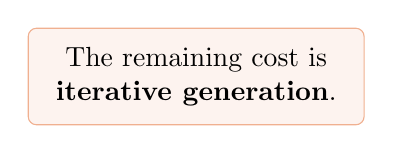
\begin{tikzpicture}
\node[draw=orange!55,fill=orange!8,rounded corners=3pt,inner xsep=10pt,inner ysep=7pt,align=center] {The remaining cost is\\\textbf{iterative generation}.};
\end{tikzpicture}
\end{columns}
\slideref{J. Ho et al., NeurIPS 2020. P. Dhariwal and A. Nichol, NeurIPS 2021. R. Rombach et al., CVPR 2022.}
\end{frame}

% 8
{
\setbeamercolor{background canvas}{bg=black}
\begin{frame}[plain]
\begin{columns}[c,onlytextwidth]
\column{0.22\textwidth}
\raggedright\color{white}\small\bfseries
``a photograph of\\[4pt]an astronaut\\[4pt]riding a horse''

\column{0.60\textwidth}
\centering
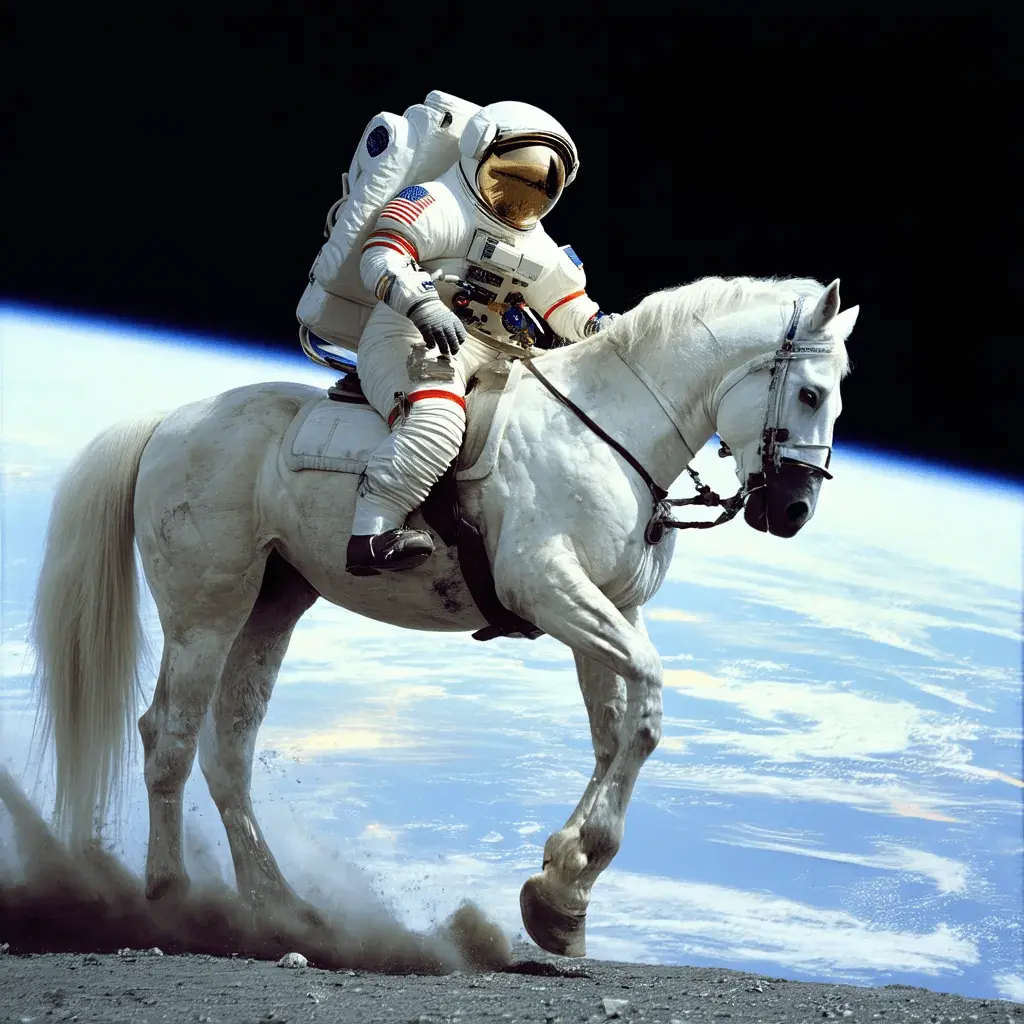
\includegraphics[width=\linewidth]{assets/stable_diffusion_astronaut_horse.png}

\column{0.14\textwidth}
\raggedright\color{white!65}\tiny
Stable Diffusion 3.5\par\smallskip
VulcanSphere\par
Wikimedia Commons\par
CC0
\end{columns}
\end{frame}
}

% 7
\begin{frame}{Diffusion is now used across the wireless stack}
\begin{columns}[T,onlytextwidth]
\column{0.34\textwidth}
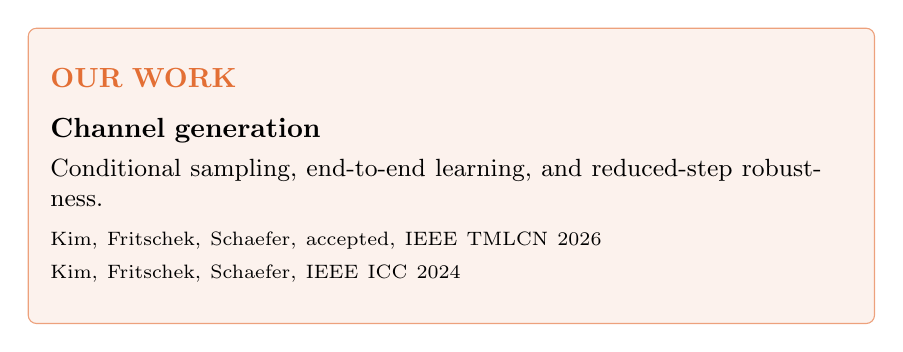
\begin{tikzpicture}
\node[draw=orange!65,fill=orange!9,rounded corners=3pt,text width=0.84\linewidth,minimum height=3.75cm,align=left,inner sep=8pt] {
\textcolor{orange}{\bfseries OUR WORK}\par\medskip
\textbf{Channel generation}\par\smallskip
\small Conditional sampling, end-to-end learning, and reduced-step robustness.\par\medskip
\scriptsize Kim, Fritschek, Schaefer, accepted, IEEE TMLCN 2026\par
Kim, Fritschek, Schaefer, IEEE ICC 2024};
\end{tikzpicture}
\column{0.31\textwidth}
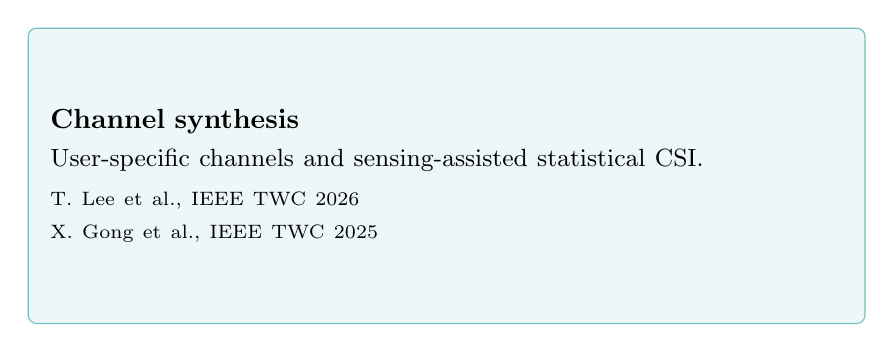
\begin{tikzpicture}
\node[draw=teal!55,fill=teal!7,rounded corners=3pt,text width=0.83\linewidth,minimum height=3.75cm,align=left,inner sep=8pt] {
\textbf{Channel synthesis}\par\smallskip
\small User-specific channels and sensing-assisted statistical CSI.\par\medskip
\scriptsize T. Lee et al., IEEE TWC 2026\par
X. Gong et al., IEEE TWC 2025};
\end{tikzpicture}
\column{0.33\textwidth}
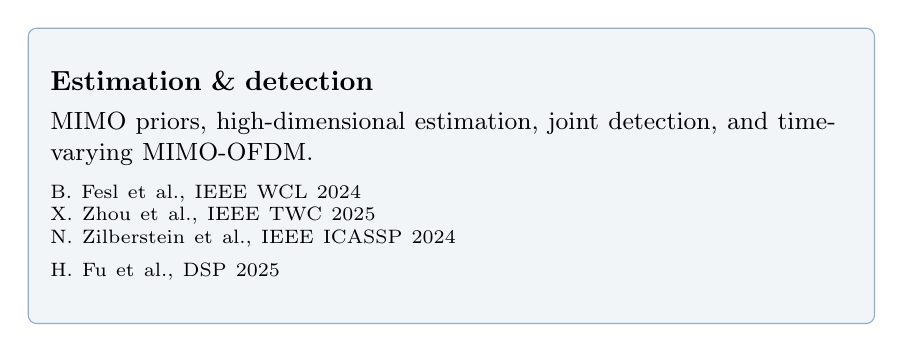
\begin{tikzpicture}
\node[draw=blue!55,fill=blue!7,rounded corners=3pt,text width=0.84\linewidth,minimum height=3.75cm,align=left,inner sep=8pt] {
\textbf{Estimation \& detection}\par\smallskip
\small MIMO priors, high-dimensional estimation, joint detection, and time-varying MIMO-OFDM.\par\medskip
\scriptsize B. Fesl et al., IEEE WCL 2024\par
X. Zhou et al., IEEE TWC 2025\par
N. Zilberstein et al., IEEE ICASSP 2024\par
H. Fu et al., DSP 2025};
\end{tikzpicture}
\end{columns}
\vspace{0.45cm}
\centering\small\color{muted} The growing application range makes sampling cost increasingly relevant.
\end{frame}

% 8
\begin{frame}{Iterative sampling turns channel calls into system cost}
\begin{columns}[T,onlytextwidth]
\column{0.52\textwidth}
\textbf{One-shot generator}\par\vspace{0.3cm}
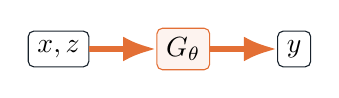
\begin{tikzpicture}[>=Latex]
\node[draw=ink,rounded corners=2pt] (z) {$x,z$};
\node[draw=orange,fill=orange!8,rounded corners=2pt,right=0.85cm of z] (g) {$G_\theta$};
\node[draw=ink,rounded corners=2pt,right=0.85cm of g] (y) {$y$};
\draw[->,line width=2pt,orange] (z)--(g); \draw[->,line width=2pt,orange] (g)--(y);
\end{tikzpicture}
\par\vspace{0.75cm}
\textbf{Diffusion generator}\par\vspace{0.3cm}
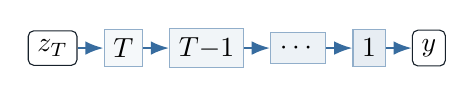
\begin{tikzpicture}[>=Latex,node distance=0.33cm]
\node[draw=ink,rounded corners=2pt] (z) {$z_T$};
\node[draw=blue!55,fill=blue!5,right=of z] (a) {$T$};
\node[draw=blue!55,fill=blue!7,right=of a] (b) {$T{-}1$};
\node[draw=blue!55,fill=blue!9,right=of b] (c) {$\cdots$};
\node[draw=blue!55,fill=blue!12,right=of c] (d) {$1$};
\node[draw=ink,rounded corners=2pt,right=of d] (y) {$y$};
\draw[->,thick,blue] (z)--(a); \draw[->,thick,blue] (a)--(b); \draw[->,thick,blue] (b)--(c); \draw[->,thick,blue] (c)--(d); \draw[->,thick,blue] (d)--(y);
\end{tikzpicture}
\column{0.44\textwidth}
\vspace{0.2cm}
\begin{block}{Where the cost appears}
\begin{itemize}\setlength\itemsep{0.55em}
\item every training mini-batch
\item every Monte Carlo sample
\item every differentiable channel call
\end{itemize}
\end{block}
\vspace{0.35cm}
\centering
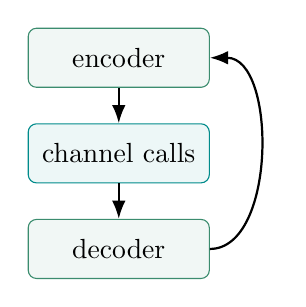
\begin{tikzpicture}[>=Latex]
\node[draw=green,fill=green!7,rounded corners=3pt,minimum width=2.3cm,minimum height=0.75cm] (tx) {encoder};
\node[draw=teal,fill=teal!7,rounded corners=3pt,minimum width=2.3cm,minimum height=0.75cm,below=0.45cm of tx] (ch) {channel calls};
\node[draw=green,fill=green!7,rounded corners=3pt,minimum width=2.3cm,minimum height=0.75cm,below=0.45cm of ch] (rx) {decoder};
\draw[->,thick] (tx)--(ch); \draw[->,thick] (ch)--(rx);
\draw[->,thick] (rx.east) .. controls ($(rx.east)+(0.85,0)$) and ($(tx.east)+(0.85,0)$) .. (tx.east);
\end{tikzpicture}
\end{columns}
\end{frame}

% 7
\begin{frame}[plain]
\centering
\vspace{1.1cm}
{\LARGE\bfseries Can we obtain direct noise-to-channel generation\par}
\vspace{0.2cm}
{\LARGE\bfseries without adversarial training and without iterative denoising?\par}
\vspace{1.0cm}
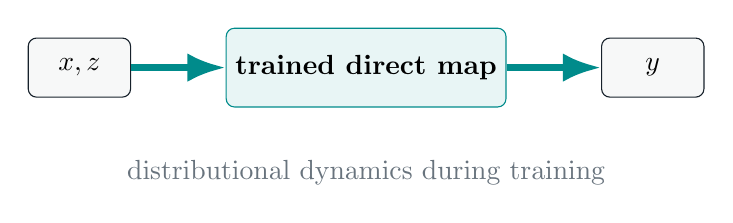
\begin{tikzpicture}[>=Latex,node distance=1.2cm]
\node[draw=ink,fill=paper,rounded corners=3pt,minimum width=1.3cm,minimum height=0.75cm] (z) {$x,z$};
\node[draw=teal,fill=teal!9,rounded corners=3pt,minimum width=3.2cm,minimum height=1.0cm,right=of z,font=\bfseries] (g) {trained direct map};
\node[draw=ink,fill=paper,rounded corners=3pt,minimum width=1.3cm,minimum height=0.75cm,right=of g] (y) {$y$};
\draw[->,line width=2.4pt,teal] (z)--(g); \draw[->,line width=2.4pt,teal] (g)--(y);
\node[below=0.55cm of g,text=muted] {distributional dynamics during training};
\end{tikzpicture}
\vfill
\hfill\color{muted}\small Drifting investigates this operating point.\hspace{0.7cm}
\end{frame}

% 10
\begin{frame}{Drifting learns a direct generator from particle directions}
\begin{columns}[T,onlytextwidth]
\column{0.31\textwidth}
\centering\textbf{1. Compare particles}\par\vspace{0.25cm}
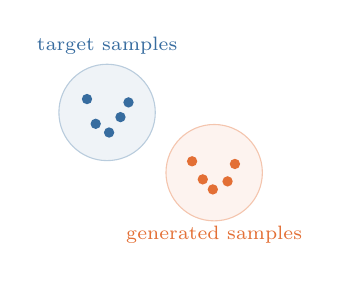
\begin{tikzpicture}[scale=0.85]
\fill[blue!8] (-0.75,0.55) circle (0.72); \draw[blue!35] (-0.75,0.55) circle (0.72);
\fill[orange!8] (0.85,-0.35) circle (0.72); \draw[orange!40] (0.85,-0.35) circle (0.72);
\foreach \x/\y in {-1.05/.75,-.72/.25,-.43/.70,-.92/.38,-.55/.48}\fill[blue] (\x,\y) circle (2.2pt);
\foreach \x/\y in {.52/-.18,.83/-.60,1.16/-.22,.68/-.45,1.05/-.48}\fill[orange] (\x,\y) circle (2.2pt);
\node[text=blue,font=\scriptsize] at (-0.75,1.55) {target samples};
\node[text=orange,font=\scriptsize] at (0.85,-1.28) {generated samples};
\end{tikzpicture}
\column{0.35\textwidth}
\centering\textbf{2. Construct a direction}\par\vspace{0.25cm}
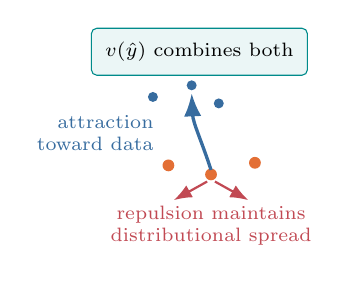
\begin{tikzpicture}[>=Latex,scale=0.82]
\node[draw=teal,fill=teal!8,rounded corners=2pt,inner sep=5pt,font=\scriptsize] at (0,1.48) {$v(\hat y)$ combines both};

% Target and generated particles occupy separate vertical bands.
\fill[blue] (-0.72,0.78) circle (2.2pt); \fill[blue] (-0.12,0.96) circle (2.2pt); \fill[blue] (0.30,0.68) circle (2.2pt);
\fill[orange] (-0.48,-0.28) circle (2.6pt); \fill[orange] (0.18,-0.42) circle (2.6pt); \fill[orange] (0.86,-0.24) circle (2.6pt);

% Attraction points from a generated particle toward the target cloud.
\draw[->,very thick,blue] (0.18,-0.35) .. controls (0.04,0.08) and (-0.10,0.38) .. (-0.12,0.84);
\node[text=blue,font=\scriptsize,align=right,anchor=east] at (-0.56,0.22) {attraction\\toward data};

% Repulsion is shown below the generated cloud to avoid crossing particles.
\draw[->,thick,red] (0.12,-0.53)--(-0.40,-0.82);
\draw[->,thick,red] (0.24,-0.53)--(0.76,-0.82);
\node[text=red,font=\scriptsize,align=center] at (0.18,-1.22) {repulsion maintains\\distributional spread};
\end{tikzpicture}
\column{0.31\textwidth}
\centering\textbf{3. Train the map}\par\vspace{0.25cm}
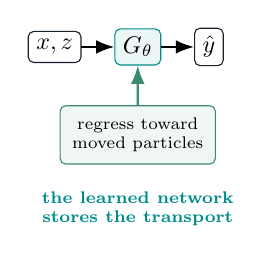
\begin{tikzpicture}[>=Latex,node distance=0.48cm,scale=0.87,transform shape]
\node[draw=ink,rounded corners=2pt] (z) {$x,z$};
\node[draw=teal,fill=teal!8,rounded corners=2pt,right=of z] (g) {$G_\theta$};
\node[draw=ink,rounded corners=2pt,right=of g] (y) {$\hat y$};
\draw[->,thick] (z)--(g); \draw[->,thick] (g)--(y);
\node[below=0.58cm of g,draw=green,fill=green!8,rounded corners=2pt,align=center,inner sep=5pt,font=\scriptsize] (u) {regress toward\\moved particles};
\draw[->,green,thick] (u)--(g);
\node[below=1.72cm of g,text=teal,font=\scriptsize\bfseries,align=center] {the learned network\\stores the transport};
\end{tikzpicture}
\end{columns}
\vspace{0.45cm}
\centering
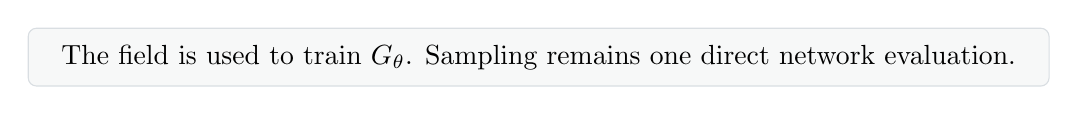
\begin{tikzpicture}\node[fill=paper,draw=line,rounded corners=3pt,inner xsep=12pt,inner ysep=6pt] {The field is used to train $G_\theta$. Sampling remains one direct network evaluation.};\end{tikzpicture}
\slideref{M. Deng et al., ``Generative Modeling via Drifting,'' arXiv:2602.04770, 2026.}
\end{frame}

% 9
\begin{frame}{A detached drift target trains the direct map}
\centering
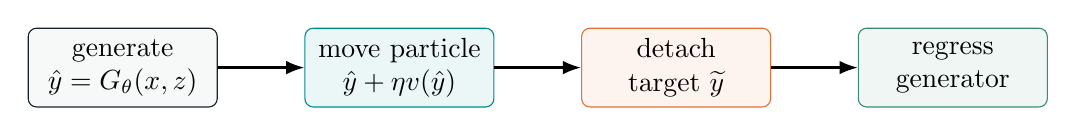
\begin{tikzpicture}[>=Latex,node distance=1.1cm]
\node[draw=ink,fill=paper,rounded corners=3pt,minimum width=2.4cm,minimum height=1.0cm,align=center] (a) {generate\\$\hat y=G_\theta(x,z)$};
\node[draw=teal,fill=teal!8,rounded corners=3pt,minimum width=2.4cm,minimum height=1.0cm,right=of a,align=center] (b) {move particle\\$\hat y+\eta v(\hat y)$};
\node[draw=orange,fill=orange!8,rounded corners=3pt,minimum width=2.4cm,minimum height=1.0cm,right=of b,align=center] (c) {detach\\target $\widetilde y$};
\node[draw=green,fill=green!8,rounded corners=3pt,minimum width=2.4cm,minimum height=1.0cm,right=of c,align=center] (d) {regress\\generator};
\draw[->,thick] (a)--(b); \draw[->,thick] (b)--(c); \draw[->,thick] (c)--(d);
\end{tikzpicture}
\vspace{0.75cm}
{\Large
\[
\widetilde y=\operatorname{stopgrad}\!\left(\hat y+\eta v(\hat y)\right),
\qquad
\min_\theta \left\|G_\theta(x,z)-\widetilde y\right\|_2^2
\]
}
\vspace{0.2cm}
\pill{blue}{CORE DESIGN CHOICE}\quad The field $v$ determines what distributional structure is learned.
\end{frame}

% 12
\begin{frame}{Repeated drift training reshapes conditional output clouds}
\centering
\includegraphics[width=0.92\textwidth]{\sourcefig{drifting_conditional_toy_figure_mpl.pdf}}
\vspace{-0.15cm}
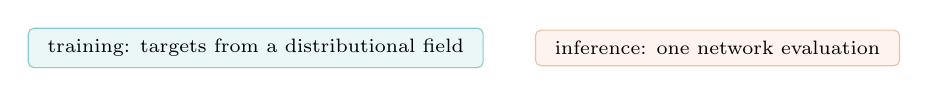
\begin{tikzpicture}[>=Latex,node distance=0.65cm]
\node[fill=teal!8,draw=teal!45,rounded corners=2pt,inner xsep=7pt,inner ysep=4pt,font=\scriptsize] (tr) {training: targets from a distributional field};
\node[fill=orange!8,draw=orange!45,rounded corners=2pt,inner xsep=7pt,inner ysep=4pt,right=of tr,font=\scriptsize] (in) {inference: one network evaluation};
\end{tikzpicture}
\slideref{Illustration follows the conditional drifting construction used in this work.}
\end{frame}

% 13
\begin{frame}{W-Flow turns Sinkhorn couplings into particle directions}
\begin{columns}[T,onlytextwidth]
\column{0.31\textwidth}
\centering\textbf{1. Couple to the target}\par\vspace{0.28cm}
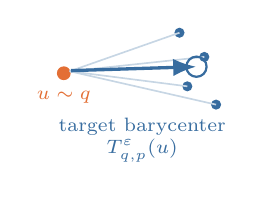
\begin{tikzpicture}[>=Latex,scale=0.83]
\fill[orange] (-1.05,0) circle (3pt);
\node[below=3pt,text=orange,font=\scriptsize] at (-1.05,0) {$u\sim q$};
\foreach \x/\y in {0.72/0.62,1.10/0.25,0.84/-0.20,1.28/-0.48}{
  \fill[blue] (\x,\y) circle (2.2pt);
  \draw[blue!28,line width=0.6pt] (-0.96,0.03)--(\x,\y);
}
\draw[blue,very thick,->] (-0.94,0.04)--(0.98,0.10);
\draw[blue,thick] (0.98,0.10) circle (4.4pt);
\node[text=blue,font=\scriptsize,align=center] at (0.15,-1.02) {target barycenter\\$T^\varepsilon_{q,p}(u)$};
\end{tikzpicture}

\column{0.31\textwidth}
\centering\textbf{2. Couple to itself}\par\vspace{0.28cm}
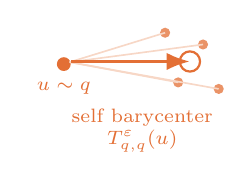
\begin{tikzpicture}[>=Latex,scale=0.83]
\fill[orange] (-1.05,0) circle (3pt);
\node[below=3pt,text=orange,font=\scriptsize] at (-1.05,0) {$u\sim q$};
\foreach \x/\y in {0.50/0.48,1.08/0.30,0.70/-0.28,1.32/-0.38}{
  \fill[orange!75] (\x,\y) circle (2.2pt);
  \draw[orange!28,line width=0.6pt] (-0.96,0.03)--(\x,\y);
}
\draw[orange,very thick,->] (-0.94,0.04)--(0.88,0.04);
\draw[orange,thick] (0.88,0.04) circle (4.4pt);
\node[text=orange,font=\scriptsize,align=center] at (0.15,-1.02) {self barycenter\\$T^\varepsilon_{q,q}(u)$};
\end{tikzpicture}

\column{0.34\textwidth}
\centering\textbf{3. Subtract the bias}\par\vspace{0.34cm}
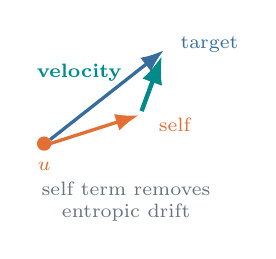
\begin{tikzpicture}[>=Latex,scale=0.86]
\fill[orange] (-1.05,-0.62) circle (3pt);
\node[below=3pt,text=orange,font=\scriptsize] at (-1.05,-0.62) {$u$};
\draw[->,very thick,blue] (-0.96,-0.56)--(0.72,0.76);
\draw[->,very thick,orange] (-0.96,-0.62)--(0.35,-0.20);
\draw[->,ultra thick,teal] (0.39,-0.14)--(0.69,0.68);
\node[text=blue,font=\scriptsize,anchor=west] at (0.82,0.84) {target};
\node[text=orange,font=\scriptsize,anchor=west] at (0.50,-0.34) {self};
\node[text=teal,font=\scriptsize\bfseries,anchor=east] at (0.24,0.43) {velocity};
\node[text=muted,font=\scriptsize,align=center] at (0.16,-1.48) {self term removes\\entropic drift};
\end{tikzpicture}
\end{columns}
\vspace{0.28cm}
\centering
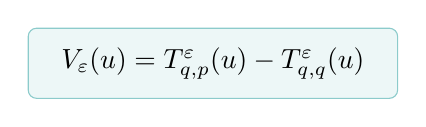
\begin{tikzpicture}
\node[draw=teal!45,fill=teal!7,rounded corners=3pt,inner xsep=12pt,inner ysep=7pt] {$V_\varepsilon(u)=T^\varepsilon_{q,p}(u)-T^\varepsilon_{q,q}(u)$};
\end{tikzpicture}
\par\vspace{0.22cm}
\small Use $u+\eta V_\varepsilon(u)$ as a detached training target; inference remains one generator evaluation.
\slideref{J. Han, P. Li, Q. Guo, R. Xu, S. Ermon, and E. J. Cand\`es, arXiv:2605.11755, 2026.}
\end{frame}

% 15
\begin{frame}{W-Flow moves one-step generation toward diffusion-level fidelity}
\centering
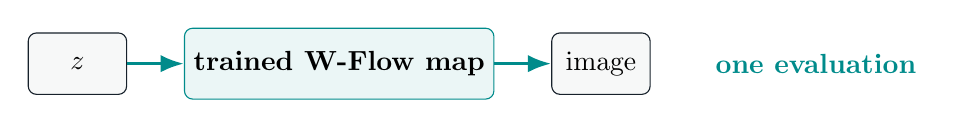
\begin{tikzpicture}[>=Latex,node distance=0.72cm]
\node[draw=ink,fill=paper,rounded corners=3pt,minimum width=1.25cm,minimum height=0.78cm] (z) {$z$};
\node[draw=teal,fill=teal!8,rounded corners=3pt,minimum width=2.65cm,minimum height=0.9cm,right=of z,font=\bfseries] (g) {trained W-Flow map};
\node[draw=ink,fill=paper,rounded corners=3pt,minimum width=1.25cm,minimum height=0.78cm,right=of g] (y) {image};
\draw[->,very thick,teal] (z)--(g); \draw[->,very thick,teal] (g)--(y);
\node[right=0.7cm of y,text=teal,font=\bfseries] {one evaluation};
\end{tikzpicture}

\vspace{0.65cm}
\begin{columns}[T,onlytextwidth]
\column{0.31\textwidth}
\centering
{\color{blue}\LARGE\bfseries 1.29}\par\smallskip
\textbf{FID}\par
\scriptsize ImageNet $256\times256$

\column{0.31\textwidth}
\centering
{\color{teal}\LARGE\bfseries $\sim100\times$}\par\smallskip
\textbf{faster sampling}\par
\scriptsize than multi-step diffusion\\at similar FID

\column{0.34\textwidth}
\centering
{\color{orange}\Large\bfseries broader coverage}\par\smallskip
\textbf{and domain transfer}\par
\scriptsize reported improvements over\\the compared one-step methods
\end{columns}

\vspace{0.60cm}
\centering\small The result motivates testing Sinkhorn-based one-step generation beyond images.
\slideref{Results reported by J. Han, P. Li, Q. Guo, R. Xu, S. Ermon, and E. J. Cand\`es, arXiv:2605.11755, 2026.}
\end{frame}

% 14
\begin{frame}{Can we apply W-Flow directly to a wireless channel?}
\begin{columns}[T,onlytextwidth]
\column{0.49\textwidth}
\centering\textbf{Correct conditional association}\par\vspace{0.2cm}
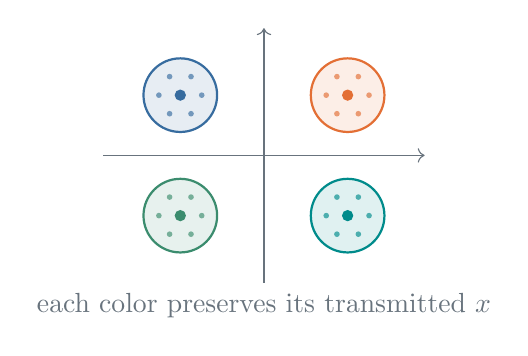
\begin{tikzpicture}[scale=0.85]
\draw[->,muted] (-2.4,0)--(2.4,0); \draw[->,muted] (0,-1.9)--(0,1.9);
\foreach \x/\y/\c in {-1.25/0.9/blue,1.25/0.9/orange,-1.25/-0.9/green,1.25/-0.9/teal}{
  \fill[\c!12] (\x,\y) circle (0.55); \draw[\c,thick] (\x,\y) circle (0.55); \fill[\c] (\x,\y) circle (2.4pt);
  \foreach \a in {0,60,...,300} \fill[\c!70] ($ (\x,\y)+(\a:0.32) $) circle (1.2pt);
}
\node[text=muted] at (0,-2.25) {each color preserves its transmitted $x$};
\end{tikzpicture}
\column{0.49\textwidth}
\centering\textbf{Same approximate marginal, wrong channel}\par\vspace{0.2cm}
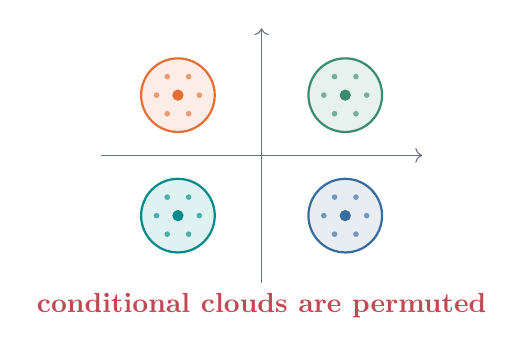
\begin{tikzpicture}[scale=0.85]
\draw[->,muted] (-2.4,0)--(2.4,0); \draw[->,muted] (0,-1.9)--(0,1.9);
\foreach \x/\y/\c in {-1.25/0.9/orange,1.25/0.9/green,-1.25/-0.9/teal,1.25/-0.9/blue}{
  \fill[\c!12] (\x,\y) circle (0.55); \draw[\c,thick] (\x,\y) circle (0.55); \fill[\c] (\x,\y) circle (2.4pt);
  \foreach \a in {0,60,...,300} \fill[\c!70] ($ (\x,\y)+(\a:0.32) $) circle (1.2pt);
}
\node[text=red,font=\bfseries] at (0,-2.25) {conditional clouds are permuted};
\end{tikzpicture}
\end{columns}
\vspace{0.15cm}
\centering
{\large $p_Y(y)=\int p(y\mid x)p_X(x)\,dx$ does not identify $p(y\mid x)$.}
\par\smallskip
\color{muted}\small We call the output cloud at fixed $x$ an \textbf{output fiber}.
\end{frame}

% 11
\begin{frame}{We adapt drifting to the conditional channel law}
\centering
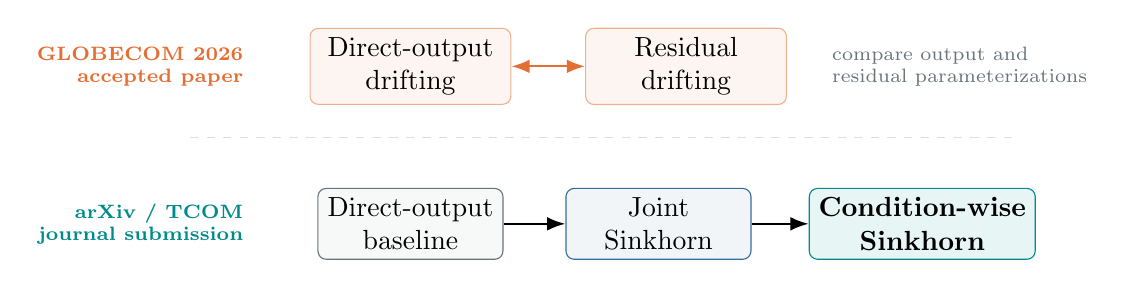
\begin{tikzpicture}[>=Latex]
\node[anchor=east,text=orange,font=\scriptsize\bfseries,align=right] at (-4.5,1.15) {GLOBECOM 2026\\accepted paper};
\node[draw=orange!55,fill=orange!7,rounded corners=3pt,minimum width=2.55cm,minimum height=0.9cm,align=center] (a) at (-2.5,1.15) {Direct-output\\drifting};
\node[draw=orange!55,fill=orange!7,rounded corners=3pt,minimum width=2.55cm,minimum height=0.9cm,align=center] (r) at (1.0,1.15) {Residual\\drifting};
\draw[<->,thick,orange] (a)--(r);
\node[right=0.45cm of r,text=muted,font=\scriptsize,align=left] {compare output and\\residual parameterizations};

\draw[line,dashed] (-5.3,0.25)--(5.2,0.25);

\node[anchor=east,text=teal,font=\scriptsize\bfseries,align=right] at (-4.5,-0.85) {arXiv / TCOM\\journal submission};
\node[draw=muted,fill=paper,rounded corners=3pt,minimum width=2.35cm,minimum height=0.9cm,align=center] (b) at (-2.5,-0.85) {Direct-output\\baseline};
\node[draw=blue,fill=blue!7,rounded corners=3pt,minimum width=2.35cm,minimum height=0.9cm,align=center] (j) at (0.65,-0.85) {Joint\\Sinkhorn};
\node[draw=teal,fill=teal!9,rounded corners=3pt,minimum width=2.55cm,minimum height=0.9cm,align=center,font=\bfseries] (c) at (4.0,-0.85) {Condition-wise\\Sinkhorn};
\draw[->,thick] (b)--(j); \draw[->,thick] (j)--(c);
\end{tikzpicture}
\vspace{0.45cm}
\begin{columns}[T,onlytextwidth]
\column{0.31\textwidth}\centering\scriptsize kernel drifting in the selected target space
\column{0.31\textwidth}\centering\scriptsize Sinkhorn transport in the joint $(x,y)$ representation
\column{0.31\textwidth}\centering\scriptsize Sinkhorn transport $y$ separately at each fixed $x$
\end{columns}
\end{frame}

% 12
\begin{frame}{Condition-wise Sinkhorn transports only the output law}
\begin{columns}[T,onlytextwidth]
\column{0.57\textwidth}
\centering
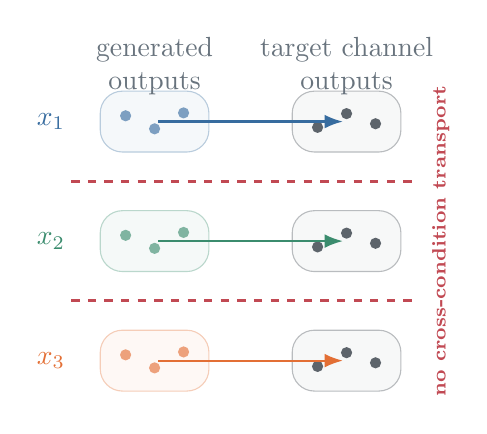
\begin{tikzpicture}[>=Latex,scale=0.92]
\foreach \row/\yy/\cc in {1/1.65/blue,2/0/green,3/-1.65/orange}{
  \node[left,text=\cc,font=\bfseries] at (-2.7,\yy) {$x_{\row}$};
  \draw[rounded corners=8pt,draw=\cc!35,fill=\cc!5] (-2.35,{\yy-0.42}) rectangle (-0.85,{\yy+0.42});
  \draw[rounded corners=8pt,draw=ink!30,fill=paper] (0.3,{\yy-0.42}) rectangle (1.8,{\yy+0.42});
  \fill[\cc!65] (-2.0,{\yy+0.08}) circle (2.2pt);
  \fill[\cc!65] (-1.6,{\yy-0.10}) circle (2.2pt);
  \fill[\cc!65] (-1.2,{\yy+0.12}) circle (2.2pt);
  \fill[ink!70] (0.65,{\yy-0.08}) circle (2.2pt);
  \fill[ink!70] (1.05,{\yy+0.11}) circle (2.2pt);
  \fill[ink!70] (1.45,{\yy-0.03}) circle (2.2pt);
  \draw[->,\cc,thick] (-1.55,\yy) -- (1.0,\yy);
}
\node[text=muted,align=center] at (-1.6,2.42) {generated\\outputs};
\node[text=muted,align=center] at (1.05,2.42) {target channel\\outputs};
\draw[red,dashed,line width=1pt] (-2.75,0.82)--(2.05,0.82);
\draw[red,dashed,line width=1pt] (-2.75,-0.82)--(2.05,-0.82);
\node[rotate=90,text=red,font=\scriptsize\bfseries] at (2.35,0) {no cross-condition transport};
\end{tikzpicture}
\column{0.41\textwidth}
\vspace{0.2cm}
\begin{block}{Conditional objective}
\[
\mathcal S^{\mathrm{cond}}_\varepsilon(q_\theta,p)
=\int \mathcal S_\varepsilon(q_{\theta,x},p_x)\,\mu(dx)
\]
\end{block}
\begin{itemize}\setlength\itemsep{0.48em}
\item repeated outputs at the same $x$
\item target coupling gives attraction
\item self coupling removes entropic bias
\item detached regression updates $G_\theta$
\end{itemize}
\end{columns}
\slideref{R. Fritschek and R. F. Schaefer, ``Condition-Wise Sinkhorn Drifting for One-Shot Learned Channel Simulation,'' arXiv:2606.17893, 2026.}
\end{frame}

% 20
\begin{frame}{The need for condition-wise Sinkhorn transport}
\centering
\includegraphics[width=0.88\textwidth,height=0.72\textheight,keepaspectratio]{\sourcefig{conditional_fiber_diagnostic_sspa.pdf}}
\vspace{-0.05cm}
\begin{columns}[onlytextwidth]
\column{0.48\textwidth}\centering\small\color{red} Joint transport displaces or collapses fixed-$x$ clouds.
\column{0.48\textwidth}\centering\small\color{teal} Condition-wise transport tracks the analytic cloud.
\end{columns}
\end{frame}

% 13
\begin{frame}{Four channels probe noise, fading, nonlinearity, and memory}
\begin{columns}[T,onlytextwidth]
\column{0.24\textwidth}
\centering\pill{blue}{AWGN}\par\vspace{0.35cm}
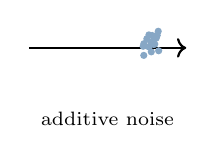
\begin{tikzpicture}\draw[->,thick] (-1,0)--(1,0); \foreach \i in {1,...,16}\fill[blue!60] ({0.45+0.22*rnd},{0.45*rnd-0.225}) circle (1.3pt); \node at (0,-0.9) {\scriptsize additive noise};\end{tikzpicture}
\column{0.24\textwidth}
\centering\pill{orange}{RAYLEIGH}\par\vspace{0.35cm}
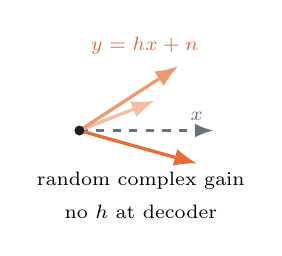
\begin{tikzpicture}[>=Latex]
\coordinate (o) at (-0.78,-0.20);
\draw[->,thick,muted,dashed] (o)--(0.92,-0.20) node[above left,text=muted,font=\scriptsize] {$x$};
\draw[->,very thick,orange!45] (o)--(0.18,0.18);
\draw[->,very thick,orange!70] (o)--(0.48,0.62);
\draw[->,very thick,orange] (o)--(0.72,-0.62);
\fill[ink] (o) circle (1.8pt);
\node[text=orange,font=\scriptsize] at (0.05,0.88) {$y=h x+n$};
\node[align=center] at (0,-1.02) {\scriptsize random complex gain\\\scriptsize no $h$ at decoder};
\end{tikzpicture}
\column{0.24\textwidth}
\centering\pill{red}{SSPA}\par\vspace{0.35cm}
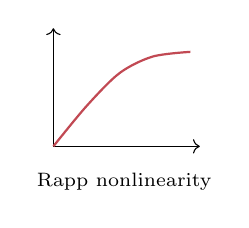
\begin{tikzpicture}[x=0.6cm,y=0.6cm]\draw[->] (0,0)--(3.1,0);\draw[->] (0,0)--(0,2.5);\draw[red,thick] plot[smooth] coordinates{(0,0)(0.7,0.85)(1.4,1.55)(2.1,1.9)(2.9,2.0)};\node at (1.5,-0.75) {\scriptsize Rapp nonlinearity};\end{tikzpicture}
\column{0.24\textwidth}
\centering\pill{teal}{TDL}\par\vspace{0.35cm}
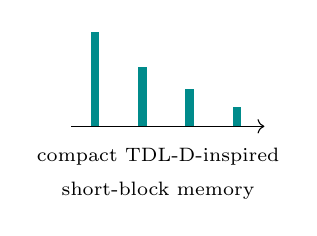
\begin{tikzpicture}\foreach \x/\h in {-0.8/1.2,-0.2/0.75,0.4/0.48,1.0/0.25}\draw[teal,line width=3pt] (\x,-0.45)--(\x,{\h-0.45}); \draw[->](-1.1,-0.45)--(1.35,-0.45); \node[align=center] at (0,-1.05) {\scriptsize compact TDL-D-inspired\\\scriptsize short-block memory};\end{tikzpicture}
\end{columns}
\vspace{0.6cm}
\centering\small AWGN $\rightarrow$ stochastic fading $\rightarrow$ nonlinear hardware $\rightarrow$ structured channel memory
\slideref{TDL profile: 3GPP TR 38.901, v17.1.0, 2022.}
\end{frame}

% 15
\begin{frame}{Condition-wise transport improves every anchor-conditioned metric}
\centering
\renewcommand{\arraystretch}{1.38}
\begin{tabular}{lcc@{\qquad}cc}
\toprule
& \multicolumn{2}{c}{Anchor SWD $\downarrow$} & \multicolumn{2}{c}{Anchor GW2 $\downarrow$}\\
Channel & Joint & Condition-wise & Joint & Condition-wise\\
\midrule
AWGN     & 0.1199 & \textbf{0.1154} & 0.4443 & \textbf{0.4277}\\
Rayleigh & 0.1723 & \textbf{0.1097} & 0.6929 & \textbf{0.3820}\\
SSPA     & 0.2174 & \textbf{0.0566} & 0.7876 & \textbf{0.2376}\\
TDL      & 0.3221 & \textbf{0.1054} & 1.1871 & \textbf{0.4444}\\
\bottomrule
\end{tabular}
\vspace{0.65cm}
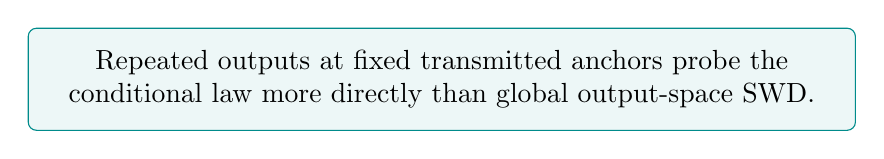
\begin{tikzpicture}
\node[draw=teal,fill=teal!7,rounded corners=3pt,inner sep=8pt,text width=0.82\textwidth,align=center] {Repeated outputs at fixed transmitted anchors probe the conditional law more directly than global output-space SWD.};
\end{tikzpicture}
\end{frame}

% 16
\begin{frame}{Downstream SER reveals both transfer and remaining gaps}
\centering
\includegraphics[width=0.94\textwidth,height=0.79\textheight,keepaspectratio]{\sourcefig{wflow_all_ser_curves.pdf}}
\end{frame}

% 17
\begin{frame}{One-shot implants use the wall clock for optimization}
\begin{columns}[T,onlytextwidth]
\column{0.56\textwidth}
\textbf{Optimizer updates in the same 1800 s budget}\par\vspace{0.4cm}
\resizebox{0.95\linewidth}{!}{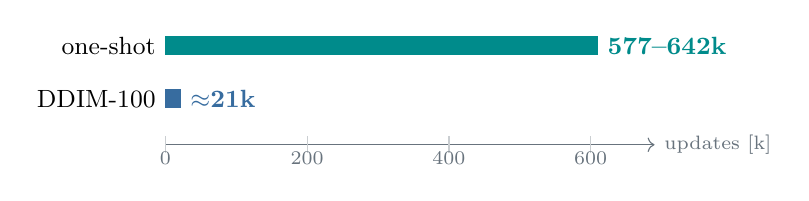
\begin{tikzpicture}[x=0.009cm,y=0.9cm]
\draw[->,muted] (0,0)--(690,0) node[right,text=muted]{\scriptsize updates [k]};
\foreach \x in {0,200,400,600}\draw[muted!35] (\x,-0.12)--(\x,0.12) node[below=2pt,text=muted]{\scriptsize\x};
\draw[line width=7pt,teal] (0,1.4)--(610,1.4); \node[left] at (0,1.4) {\small one-shot}; \node[right,text=teal,font=\bfseries] at (610,1.4) {\small 577--642k};
\draw[line width=7pt,blue] (0,0.65)--(21.5,0.65); \node[left] at (0,0.65) {\small DDIM-100}; \node[right,text=blue,font=\bfseries] at (21.5,0.65) {\small $\approx$21k};
\end{tikzpicture}}
\vspace{0.55cm}
\small Same symbolic autoencoder; final evaluation uses the analytic channel. Mean over 30 seeds.
\column{0.40\textwidth}
\textbf{Lowest learned SER under this budget}\par\vspace{0.3cm}
\scriptsize
\renewcommand{\arraystretch}{1.45}
\begin{tabular}{ll}
\toprule
AWGN & \textcolor{teal}{Condition-wise Sinkhorn}\\
Rayleigh & \textcolor{blue}{DDIM-100}\\
SSPA & \textcolor{teal}{Condition-wise Sinkhorn}\\
TDL & \textcolor{orange}{WGAN}\\
\bottomrule
\end{tabular}
\par\vspace{0.45cm}
\color{muted}\small The method ranking remains channel-dependent.
\end{columns}
\end{frame}

% 18
\begin{frame}{The best operating point depends on how the simulator is used}
\textbf{Measured inference time per sample on an NVIDIA RTX 5060 Ti}\par\vspace{0.35cm}
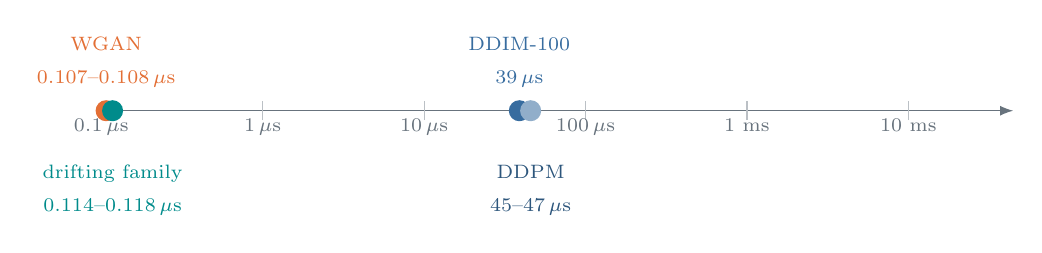
\begin{tikzpicture}[x=2.05cm,y=1cm,>=Latex]
\draw[->,muted] (0,0)--(5.65,0);
\foreach \x/\lab in {0/$0.1\,\mu$s,1/$1\,\mu$s,2/$10\,\mu$s,3/$100\,\mu$s,4/$1$ ms,5/$10$ ms}{\draw[muted!45] (\x,-0.12)--(\x,0.12) node[below=3pt,text=muted]{\scriptsize\lab};}
\fill[orange] (0.03,0) circle (3.8pt); \node[above=5pt,text=orange,align=center] at (0.03,0) {\scriptsize WGAN\\\scriptsize $0.107$--$0.108\,\mu$s};
\fill[teal] (0.07,0) circle (3.8pt); \node[below=16pt,text=teal,align=center] at (0.07,0) {\scriptsize drifting family\\\scriptsize $0.114$--$0.118\,\mu$s};
\fill[blue] (2.59,0) circle (3.8pt); \node[above=5pt,text=blue,align=center] at (2.59,0) {\scriptsize DDIM-100\\\scriptsize $39\,\mu$s};
\fill[blue!55] (2.66,0) circle (3.8pt); \node[below=16pt,text=blue!70!ink,align=center] at (2.66,0) {\scriptsize DDPM\\\scriptsize $45$--$47\,\mu$s};
\end{tikzpicture}
\vspace{0.75cm}
\begin{columns}[T,onlytextwidth]
\column{0.48\textwidth}
\begin{block}{Standalone fidelity dominates}
Diffusion can justify sequential sampling on the harder final SER curves.
\end{block}
\column{0.48\textwidth}
\begin{block}{Repeated channel calls dominate}
One-shot generators preserve more time for system optimization and simulation.
\end{block}
\end{columns}
\end{frame}

% 26
\begin{frame}{Open problems: time variation, nonlinearity, and MIMO}
\begin{columns}[T,onlytextwidth]
\column{0.32\textwidth}
\centering\pill{blue}{TIME VARIATION}\par\vspace{0.34cm}
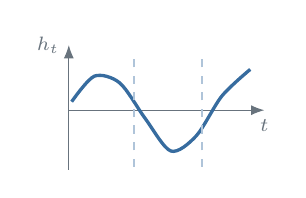
\begin{tikzpicture}[x=0.72cm,y=0.72cm,>=Latex]
\draw[->,muted] (0,0)--(3.45,0) node[below,font=\scriptsize] {$t$};
\draw[->,muted] (0,-1.05)--(0,1.15) node[left,font=\scriptsize] {$h_t$};
\draw[blue,very thick,smooth] plot coordinates {(0.05,0.15)(0.45,0.60)(0.90,0.48)(1.35,-0.15)(1.80,-0.72)(2.25,-0.45)(2.70,0.25)(3.20,0.72)};
\draw[blue!40,dashed] (1.15,-1.0)--(1.15,1.0);
\draw[blue!40,dashed] (2.35,-1.0)--(2.35,1.0);
\end{tikzpicture}
\vspace{0.18cm}
\textbf{Channels evolve during use}\par\smallskip
\scriptsize Doppler, nonstationarity, and long temporal memory

\column{0.32\textwidth}
\centering\pill{red}{NONLINEARITY}\par\vspace{0.34cm}
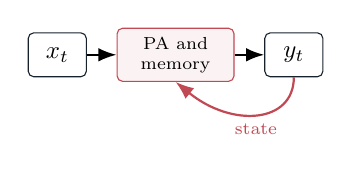
\begin{tikzpicture}[>=Latex,node distance=0.42cm,scale=0.90,transform shape]
\node[draw=ink,rounded corners=2pt,minimum width=0.82cm,minimum height=0.62cm] (x) {$x_t$};
\node[draw=red,fill=red!7,rounded corners=2pt,minimum width=1.65cm,minimum height=0.75cm,right=of x,align=center,font=\scriptsize] (pa) {PA and\\memory};
\node[draw=ink,rounded corners=2pt,minimum width=0.82cm,minimum height=0.62cm,right=of pa] (y) {$y_t$};
\draw[->,thick] (x)--(pa); \draw[->,thick] (pa)--(y);
\draw[->,red,thick] (y.south) .. controls +(0,-0.65) and +(0.8,-0.65) .. node[below,font=\scriptsize,text=red] {state} (pa.south);
\end{tikzpicture}
\vspace{0.52cm}
\textbf{Stateful distortion}\par\smallskip
\scriptsize Dynamic amplifiers, coupled impairments, and wider operating ranges

\column{0.32\textwidth}
\centering\pill{teal}{SPATIAL STRUCTURE}\par\vspace{0.28cm}
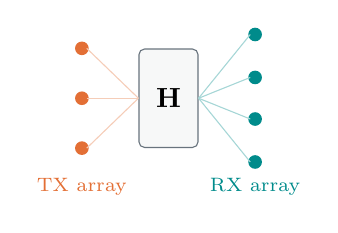
\begin{tikzpicture}[>=Latex,scale=0.88]
\foreach \y in {-0.72,0,0.72}{\fill[orange] (-1.25,\y) circle (2.8pt);}
\foreach \y in {-0.92,-0.30,0.30,0.92}{\fill[teal] (1.25,\y) circle (2.8pt);}
\node[draw=muted,fill=paper,rounded corners=2pt,minimum width=0.75cm,minimum height=1.25cm] (h) at (0,0) {$\mathbf H$};
\foreach \a in {-0.72,0,0.72}{\draw[orange!35] (-1.18,\a)--(h.west);}
\foreach \b in {-0.92,-0.30,0.30,0.92}{\draw[teal!35] (h.east)--(1.18,\b);}
\node[text=orange,font=\scriptsize] at (-1.25,-1.28) {TX array};
\node[text=teal,font=\scriptsize] at (1.25,-1.28) {RX array};
\end{tikzpicture}
\vspace{0.20cm}
\textbf{Dimension grows quickly}\par\smallskip
\scriptsize MIMO correlation, array geometry, and environment state
\end{columns}
\vspace{0.55cm}
\centering
\begin{tikzpicture}
\node[draw=teal!45,fill=teal!7,rounded corners=3pt,inner xsep=12pt,inner ysep=7pt] {Goal: preserve $p(y\mid x)$ as dimension, memory, and channel state grow.};
\end{tikzpicture}
\end{frame}

% 19
\begin{frame}{Design channel generators for fidelity, structure, and cost together}
\begin{columns}[T,onlytextwidth]
\column{0.68\textwidth}
\small
\begin{enumerate}\setlength\itemsep{0.8em}
\item[\textcolor{blue}{\bfseries 1.}] \textbf{Generative models provide flexible learned wireless channel simulators.}
\item[\textcolor{orange}{\bfseries 2.}] \textbf{Diffusion offers strong distributional modeling, but iterative sampling can be costly.}
\item[\textcolor{teal}{\bfseries 3.}] \textbf{Conditional drifting explores direct generation without adversarial training.}
\end{enumerate}
\column{0.30\textwidth}
\centering
\begin{tikzpicture}[scale=0.72,transform shape]
\coordinate (a) at (90:1.65); \coordinate (b) at (210:1.65); \coordinate (c) at (330:1.65);
\draw[very thick,line] (a)--(b)--(c)--cycle;
\fill[blue] (a) circle (4pt); \fill[orange] (b) circle (4pt); \fill[teal] (c) circle (4pt);
\node[above,text=blue,font=\bfseries] at (a) {fidelity};
\node[below left,text=orange,font=\bfseries] at (b) {structure};
\node[below right,text=teal,font=\bfseries] at (c) {cost};
\node[align=center] at (0,0) {learned\\channel};
\end{tikzpicture}
\end{columns}
\vfill
\centering\color{muted}\small Conditioning remains critical. Structured, high-dimensional, and measured channels remain open challenges.
\end{frame}

\appendix

% B1
\begin{frame}{Backup: Generic drifting uses attraction and repulsion}
\small
For generated particles $g_i$ and target particles $p_j$, the direct-output field is
\[
V(g_i)=\left(\sum_j w^P_{ij}p_j-g_i\right)
-\lambda\left(\sum_k w^G_{ik}g_k-g_i\right),
\]
where $w^P$ and $w^G$ are row-normalized radial-basis-function kernel weights.
\vspace{0.2cm}
\[
\widetilde g_i=\operatorname{stopgrad}\!\left(g_i+\eta V(g_i)\right),
\qquad
\mathcal L_\theta=\frac1B\sum_i\|f_\theta(z_i)-\widetilde g_i\|_2^2.
\]
\begin{columns}[T,onlytextwidth]
\column{0.48\textwidth}\softbox{blue}{\centering Attraction moves particles toward target samples.}
\column{0.48\textwidth}\softbox{orange}{\centering Repulsion discourages generated-particle collapse.}
\end{columns}
\end{frame}

% B2
\begin{frame}{Backup: Optimal transport matches probability mass globally}
\small
For empirical laws
\[
q=\sum_{i=1}^{n}a_i\delta_{u_i},
\qquad
p=\sum_{j=1}^{m}b_j\delta_{v_j},
\qquad
\sum_i a_i=\sum_j b_j=1,
\]
a coupling is a nonnegative transport matrix with the prescribed marginals:
\[
\Pi(a,b)=\left\{\pi\in\mathbb R_+^{n\times m}:\;
\pi\mathbf 1_m=a,\quad \pi^\mathsf T\mathbf 1_n=b\right\}.
\]
Optimal transport selects the least-cost admissible coupling,
\[
\operatorname{OT}_c(q,p)
=\min_{\pi\in\Pi(a,b)}\sum_{i,j}\pi_{ij}\,c(u_i,v_j).
\]
\begin{columns}[T,onlytextwidth]
\column{0.48\textwidth}\softbox{blue}{\centering $\pi_{ij}$ is the mass transported from $u_i$ to $v_j$.}
\column{0.48\textwidth}\softbox{teal}{\centering For $c(u,v)=\lVert u-v\rVert_2^2$, this cost gives $W_2^2(q,p)$.}
\end{columns}
\end{frame}

% B3
\begin{frame}{Backup: Entropic OT produces the W-Flow velocity}
\footnotesize
Sinkhorn iterations solve the regularized transport problem
\vspace{-0.08cm}
\[
\operatorname{OT}_\varepsilon(q,p)
=\min_{\pi\in\Pi(a,b)}
\left\{\sum_{i,j}\pi_{ij}c(u_i,v_j)
+\varepsilon\operatorname{KL}(\pi\,\|\,a\otimes b)\right\}.
\]
\vspace{-0.14cm}
Subtracting the two self-costs removes entropic bias:
\vspace{-0.08cm}
\[
\mathcal S_\varepsilon(q,p)=\operatorname{OT}_\varepsilon(q,p)
-\tfrac12\operatorname{OT}_\varepsilon(q,q)
-\tfrac12\operatorname{OT}_\varepsilon(p,p).
\]
\vspace{-0.14cm}
The target coupling defines a barycentric transport map,
\vspace{-0.08cm}
\[
T^\varepsilon_{q,p}(u_i)=\frac{1}{a_i}\sum_j\pi^\star_{ij}v_j.
\]
\vspace{-0.14cm}
Hence the empirical particle velocity is
\vspace{-0.08cm}
\[
V_\varepsilon(u)=T^\varepsilon_{q,p}(u)-T^\varepsilon_{q,q}(u).
\]
\vspace{-0.10cm}
\begin{columns}[T,onlytextwidth]
\column{0.48\textwidth}\softbox{teal}{\centering Target coupling: attraction toward the data barycenter.}
\column{0.48\textwidth}\softbox{orange}{\centering Self coupling: entropic-bias correction and repulsion.}
\end{columns}
\vspace{0.03cm}
\centering\footnotesize Main experiments: 10 Sinkhorn iterations; minimum $\varepsilon=10^{-3}$.
\end{frame}

% B4
\begin{frame}{Backup: The conditional objective has the desired population equilibrium}
\small
With shared input marginal $\mu$,
\[
p(dx,dy)=\mu(dx)p_x(dy),\qquad q_\theta(dx,dy)=\mu(dx)q_{\theta,x}(dy).
\]
Define
\[
\mathcal S^{\mathrm{cond}}_\varepsilon(q_\theta,p)
=\int \mathcal S_\varepsilon(q_{\theta,x},p_x)\,\mu(dx).
\]
Under the standard Sinkhorn-divergence assumptions,
\[
\mathcal S^{\mathrm{cond}}_\varepsilon(q_\theta,p)=0
\quad\Longleftrightarrow\quad
q_{\theta,x}=p_x\quad\text{for $\mu$-almost every }x.
\]
\vspace{0.3cm}
\alert{Scope:} This is a population statement. Finite minibatch barycentric velocities and detached neural-network regression are practical approximations, especially under model misspecification.
\end{frame}

% B5
\begin{frame}{Backup: The estimator uses repeated outputs per transmitted input}
\begin{columns}[T,onlytextwidth]
\column{0.55\textwidth}
For each anchor $x_b$:
\begin{enumerate}\setlength\itemsep{0.42em}
\item Draw $K_g=4$ generated outputs.
\item Draw $K_p=4$ target channel outputs.
\item Draw $K_r=4$ independent generated references.
\item Solve target and self Sinkhorn problems in output space.
\item Regress toward the detached barycentric velocity target.
\end{enumerate}
\column{0.41\textwidth}
\begin{block}{Leading coupling cost}
\small
Condition-wise:
\[
O\!\left(IBK_g(K_p+K_r)\right)
\]
Expanded joint batch:
\[
O\!\left(IB^2K_g(K_p+K_r)\right)
\]
\end{block}
\end{columns}
\vspace{0.35cm}
\centering\color{muted}\small At inference, both variants use one evaluation of the same generator architecture.
\end{frame}

% B6
\begin{frame}{Backup: Condition-wise Sinkhorn training update}
\footnotesize
\softbox{blue}{\textbf{Input:} generator $g_\theta$, channel sampler $p(\cdot\mid x)$, anchors $x_i$, counts $K_g,K_p,K_r$, and drift scale $\eta$.}
\vspace{0.14cm}
\begin{columns}[T,onlytextwidth]
\column{0.47\textwidth}
\textbf{Sample at each fixed $x_i$}
\begin{enumerate}\setlength\itemsep{0.48em}
\item Generated particles:
\[
\hat y_{i,k}=g_\theta(x_i,z_{i,k}),\quad k=1{:}K_g.
\]
\item Positive channel samples:
\[
y_{i,j}\sim p(\cdot\mid x_i),\quad j=1{:}K_p.
\]
\item Independent generated references:
\[
\hat y'_{i,\ell}=g_\theta(x_i,z'_{i,\ell}),\quad \ell=1{:}K_r.
\]
\end{enumerate}
\column{0.49\textwidth}
\textbf{Transport and project}
\begin{enumerate}\setcounter{enumi}{3}\setlength\itemsep{0.48em}
\item Solve, separately for every $i$,
\[
\hat Q_i\leftrightarrow P_i,\qquad
\hat Q_i\leftrightarrow\hat Q'_i.
\]
\item Form the barycentric velocity:
\[
v_{i,k}=T^\varepsilon_{\hat Q_i,P_i}(\hat y_{i,k})
-T^\varepsilon_{\hat Q_i,\hat Q'_i}(\hat y_{i,k}).
\]
\item Update $\theta$ by regressing toward
\[
\operatorname{stopgrad}(\hat y_{i,k}+\eta v_{i,k}).
\]
\end{enumerate}
\end{columns}
\vspace{0.06cm}
\centering\color{muted} Repeat during training. Afterward, sampling is the direct map $\hat y=g_\theta(x,z)$.
\end{frame}

% B7
\begin{frame}{Backup: Direct-output SWD gives a different ranking}
\scriptsize
\centering
\renewcommand{\arraystretch}{1.25}
\begin{tabular}{lcccc}
\toprule
Method & AWGN & Rayleigh & SSPA & TDL\\
\midrule
WGAN & $.0198\pm.0050$ & $.0171\pm.0050$ & $.0287\pm.0156$ & $.0289\pm.0063$\\
DDPM & $.0070\pm.0004$ & $.0079\pm.0008$ & $.0032\pm.0005$ & $.0297\pm.0011$\\
DDIM-100 & $.0042\pm.0006$ & $.0044\pm.0007$ & $.0024\pm.0004$ & $.0248\pm.0009$\\
\midrule
Direct drifting & $.0100\pm.0007$ & $.0085\pm.0012$ & $\mathbf{.0060\pm.0008}$ & --\\
Joint Sinkhorn & $.0148\pm.0002$ & $.0152\pm.0002$ & $.0117\pm.0002$ & $.0966\pm.0005$\\
Condition-wise Sinkhorn & $\mathbf{.0058\pm.0001}$ & $\mathbf{.0073\pm.0001}$ & $.0071\pm.0002$ & $\mathbf{.0118\pm.0002}$\\
\bottomrule
\end{tabular}
\vspace{0.45cm}
\begin{minipage}{0.9\textwidth}
\small Reference WGAN/diffusion rows use their stable benchmark protocols. The drifting-family block is the controlled matched-architecture comparison; bold marks its best value. Reference runs use 10 seeds, W-Flow rows use 100 seeds, and the SSPA condition-wise row uses the 30-seed update-budget-controlled run.
\end{minipage}
\end{frame}

% B8
\begin{frame}{Backup: SSPA requires an update-budget-controlled operating point}
\scriptsize
\centering
\renewcommand{\arraystretch}{1.3}
\begin{tabular}{lrrrrrr}
\toprule
Run & Updates & Seeds & Direct SWD & Anchor-SWD ratio & Anchor-GW2 ratio & SER at 8 dB\\
\midrule
Short local & 0.31k & 1 & $1.07\!\times\!10^{-1}$ & 5.14 & 4.10 & --\\
Early compact & 0.88k & 1 & $4.09\!\times\!10^{-2}$ & 4.50 & 3.88 & --\\
Reported point & 4.69k & 30 & $7.07\!\times\!10^{-3}$ & 1.13 & 1.15 & $9.33\!\times\!10^{-5}$\\
Full preset & 390.6k & 100 & $1.53$ & 35.5 & 60.1 & $2.70\!\times\!10^{-2}$\\
\bottomrule
\end{tabular}
\vspace{0.45cm}
\begin{minipage}{0.92\textwidth}
\small Ratios divide learned-versus-analytic anchor metrics by an analytic-versus-analytic floor from independent channel draws. The sharp same-condition field converges early; with fixed drift scale and small same-condition sample sets, the long diffusion-style preset is a poor long-horizon optimizer. The full-preset row is a sensitivity check and is not used for model selection.
\end{minipage}
\end{frame}

% B9
\begin{frame}{Backup: The AWGN result transfers to block length 64}
\begin{columns}[T,onlytextwidth]
\column{0.67\textwidth}
\centering
\includegraphics[width=\textwidth,height=0.72\textheight,keepaspectratio]{\sourcefig{turboae_awgn_l64_ber_bler_curve_eval2k.pdf}}
\column{0.30\textwidth}
\vspace{0.55cm}
\textbf{TurboAE-style check}
\begin{itemize}\setlength\itemsep{0.38em}
\item block length 64
\item rate $1/2$
\item training at 4 dB
\item 30 seeds
\item analytic evaluation
\end{itemize}
\vspace{0.35cm}
\textbf{BER at 4 dB}
\begin{itemize}\setlength\itemsep{0.35em}
\item analytic: $1.96\times10^{-3}$
\item condition-wise: $3.30\times10^{-3}$
\end{itemize}
\end{columns}
\end{frame}

% B10
\begin{frame}{Backup: Scope and reproducibility boundaries}
\begin{columns}[T,onlytextwidth]
\column{0.48\textwidth}
\textbf{Controlled conclusions}
\begin{itemize}\setlength\itemsep{0.38em}
\item W-Flow variants share the same one-shot generator.
\item Drift-field differences drive their ablation ranking.
\item Cross-family baselines use stable reference protocols.
\item Comparisons are contextual, not fully matched capacity.
\end{itemize}
\column{0.48\textwidth}
\textbf{Current limitations}
\begin{itemize}\setlength\itemsep{0.38em}
\item exact estimator assumes repeated outputs at fixed $x$
\item local measured-data approximation is not yet validated
\item compact TDL is not a full OFDM-scale evaluation
\item global SWD must be paired with conditional and downstream metrics
\end{itemize}
\end{columns}
\vspace{0.55cm}
\begin{block}{Timing protocol}
\small PyTorch float32 on NVIDIA RTX 5060 Ti; batch size 512; CUDA synchronization; no graph capture, compilation, or mixed precision. Source code: \texttt{github.com/Fritschek/conditional\_drifting\_models\_public}
\end{block}
\end{frame}

% B11
\begin{frame}{Backup: Inference-network parameter counts}
\scriptsize
\centering
\renewcommand{\arraystretch}{1.3}
\begin{tabular}{lrrrr}
\toprule
Model & AWGN & Rayleigh & SSPA & TDL\\
\midrule
Direct drifting & 20,487 & 20,487 & 20,744 & 20,744\\
Sinkhorn drifting variants & 20,487 & 20,487 & 20,744 & 20,744\\
Diffusion denoiser & 59,847 & 74,247 & 60,178 & 74,632\\
WGAN generator & 19,335 & 71,431 & 72,200 & 72,200\\
\bottomrule
\end{tabular}
\vspace{0.55cm}
\begin{minipage}{0.9\textwidth}
\small Sinkhorn couplings are training-time computations and add no inference-time parameters. DDPM and DDIM share denoiser weights. Cross-family architectures and training schedules follow stable family-specific protocols rather than a fully matched-capacity design.
\end{minipage}
\end{frame}

% B12
\begin{frame}{Backup: Selected references}
\scriptsize
\begin{itemize}\setlength\itemsep{0.35em}
\item I. Goodfellow et al., ``Generative Adversarial Nets,'' NeurIPS, 2014.
\item M. Arjovsky, S. Chintala, and L. Bottou, ``Wasserstein Generative Adversarial Networks,'' ICML, 2017.
\item J. Ho, A. Jain, and P. Abbeel, ``Denoising Diffusion Probabilistic Models,'' NeurIPS, 2020.
\item P. Dhariwal and A. Nichol, ``Diffusion Models Beat GANs on Image Synthesis,'' NeurIPS, 2021.
\item J. Song, C. Meng, and S. Ermon, ``Denoising Diffusion Implicit Models,'' ICLR, 2021.
\item R. Rombach et al., ``High-Resolution Image Synthesis with Latent Diffusion Models,'' CVPR, 2022.
\item M. Kim, R. Fritschek, and R. F. Schaefer, ``Diffusion Models for Accurate Channel Distribution Generation,'' accepted, IEEE TMLCN, 2026.
\item M. Kim, R. Fritschek, and R. F. Schaefer, ``Robust Generation of Channel Distributions with Diffusion Models,'' IEEE ICC, 2024.
\item M. Deng, H. Li, T. Li, Y. Du, and K. He, ``Generative Modeling via Drifting,'' arXiv:2602.04770, 2026.
\item J. Han et al., ``One-Step Generative Modeling via Wasserstein Gradient Flows,'' arXiv:2605.11755, 2026.
\item R. Fritschek and R. F. Schaefer, ``Condition-Wise Sinkhorn Drifting for One-Shot Learned Channel Simulation,'' arXiv:2606.17893, 2026.
\item M. Cuturi, ``Sinkhorn Distances: Lightspeed Computation of Optimal Transport,'' NeurIPS, 2013.
\item J. Feydy et al., ``Interpolating between Optimal Transport and MMD using Sinkhorn Divergences,'' AISTATS, 2019.
\end{itemize}
\end{frame}

\end{document}
